\section{Realisation}

Mit der im vorangegangenen Abschnitt beschriebenen Architektur und den aufgestellten Leistungsanforderungen, wird im folgenden Abschnitt die Umsetzung der Beispielapplikation, die dafür genutzten Werkzeuge und notwendige Anpassungen beschrieben. Der Fokus liegt dabei auf den Bestandteilen die direkt bei der Personallisierung der Suche genutzt werden.

Ausgangspunkt bei der Umsetzung war die bereits vorhandene \textit{Searchperience} Suchlösung welche entsprechend der Anforderungen angepasst werden sollte.
Da \textit{Searchperience} das Java basierte Apache Solr zum Aufbau und zur Abfrage der Suchindexe nutzt, wurden für die weiteren Bestandteile ebenfalls Java-Bibliotheken genutzt.

\subsection{Apache Solr}\label{sec:solr}

Apache Solr (Solr) ist ein ``Enterprise Search Server'' welcher unter der Apache 2.0 Lizenz frei zur Verfügung steht. Aufbauend auf der Apache Lucene Suchbibliothek ermöglicht Solr den Aufbau einer sehr vielfältig konfigurierbaren Volltextsuche. Zu den wichtigsten Konfigurations- und Erweiterungseigenschaften zählen facettierte Suchen, automatische Anfragevervollständigung, dynamische Relevanz-Anpassungen (Boosting), Indexreplikation und Indexsharding (vgl. Abschnitt \ref{sec:sharding}). Genutzt werden kann Apache Solr über eine \glslink{REST}{``RESTful HTTP''} Schnittstelle, welche sowohl XML als auch \gls{JSON} zum Datenaustausch nutzten kann.

\paragraph{Konfiguration} Die zwei wichtigsten Quellen zur Konfiguration des Dienstes sind die \textit{solrconfig.xml} und die \textit{schema.xml}. Die \textit{solrconfig.xml} dient zur Integration aller Komponenten und integriert die Bestandteile und der Schnittstellen. Sie bestimmt zum Beispiel in welcher Reihenfolge und mit welchen Voreinstellungen die einzelnen Komponenten eine Suchanfrage bearbeiten und ermöglicht daneben auch die Integration eigener Komponenten. Mit Hilfe der  \textit{schema.xml} werden die vom Server verwalteten Dokumente bzw. Dokumentenbestandteile beschrieben und notwendige Vorverarbeitungsschritte konfiguriert. Kommentierte Beispiel- bzw. Basiskonfigurationen der beiden Konfigurationsdateien\footnote{\tiny{http://svn.apache.org/viewvc/lucene/dev/trunk/solr/example/solr/collection1/conf/solrconfig.xml?view=markup}}\textsuperscript{,}\footnote{\tiny{http://svn.apache.org/viewvc/lucene/dev/trunk/solr/example/solr/collection1/conf/schema.xml?view=markup}}, sowie die Dokumentation der Anfragesyntax\footnote{\tiny{Anfragesyntax: http://wiki.apache.org/solr/ExtendedDisMax}}\textsuperscript{,}\footnote{\tiny{Anfrage-Funktionen: http://wiki.apache.org/solr/FunctionQuery}} sind ebenfalls Bestandteil der offenen Quelltexte und werden hier zur Wahrung des Umfangs nur kurz beschrieben.

\subsubsection{Datenhaltung}

Da Dokumente selten aus fortlaufendem unstrukturierten Text bestehen, oftmals ergänzende Informationen zu einem Dokument im Suchindex verfügbar gemacht werden sollen und da die Datenhalten möglichst effizient geschehen soll, ist es notwendig die mögliche Struktur der Daten mit Hilfe der \textit{schema.xml} zu beschrieben. Um Redundanz innerhalb der Strukturbeschreibung zu vermeiden ist diese zweigeteilt. Zunächst werden alle Datentypen (\textit{types}) konfiguriert -- d.h. aus der Liste der möglichen Standardtypen werden die für den Anwendungsfall notwendigen ausgewählt und ggf. mit angepasster Basiskonfiguration verfügbar gemacht. Eine detailliertere Unterscheidung der Typen ist notwendig um sicherzustellen, dass die Daten möglichst effizient für den konkreten Anwendungsfall gespeichert werden. Im zweiten Schritt werden dann die eigentlichen Dokumentenbestandteile (auch Felder oder \textit{fields}) den vorher konfigurierten Typen zugeordnet. In einer auf einen einzelnen Typen und ein Feld reduzierten Form zeigt Listing \ref{lst:schema_vektor} dies beispielhaft. Anhand der Konfiguration werden die vorgehaltenen Dokumente mit Hilfe der geeigneten invertierten Indexe (vgl. Abschnitt \ref{sec:indexcreation}) organisiert.

\lstinputlisting[caption=Instanzierung von Apache Solr zur horizontalen Skalierung,label={lst:solrsharding},float]{Listings/solr_sharding.txt}

Die horizontale Skalierung (vgl. Abschnitt \ref{sec:sharding}) der in Solr vorgehaltenen Daten kann über beliebig viele \textit{Backend-Knoten} erfolgen. Dabei werden, wie in Listing \ref{lst:solrsharding}, die einzelnen Solr-Instanzen mit einer Referenz auf eine zentrale Konfigurationsinstanz gestartet (im Beispiel über Apache Zookeeper). Die Wahl der Server-Rollen (Frontend- o. Backend) erfolgt je nach Verfügbarkeit und wird automatisch erneutert wenn Knoten ausfallen oder ergänzt werden. Mögliche Redundanz in der Datenhaltung, und damit die Steigerung der Leistungsfähigkeit von Leseoperationen, kann durch du die Konfiguration der insgesamt genutzten Datenblöcke (auch \textit{Shards}), den Replikations-Faktor und die Datenblöcke pro Knoten erzielt werden.

\subsubsection{Suchanfragen}

Innerhalb von Solr können sog. \textit{RequestHandler} genutzt werden um Daten aus dem Index zu lesen, bzw. um Suchen innerhalb der Dokumentensammlung durchzuführen. Jeder \textit{RequestHandler} ist wiederum aus verschiedenen Komponenten aufgebaut welche innerhalb der \textit{solrconfig.xml} konfiguriert bzw. ergänzt werden können.

Die Komponenten innerhalb der Konfiguration spiegeln auch die Verarbeitungsreihenfolge der Suchanfragen wieder. Die Standardkomponenten des \textit{SearchHandler} sind \texttt{solr.QueryComponent} (Query), \texttt{solr.FacetComponent} (Facet), \texttt{solr.MoreLikeThisComponent} (Mlt), \texttt{solr.HighlightComponent} (Highlight) und \texttt{solr.HighlightComponent} (Stats). Innerhalb einer Suchanfrage wird in \texttt{Query} die eigentliche Ergebnisliste gebildet welche dann im folgenden gefiltert (\texttt{Facet}), ergänzt (\texttt{Mlt}) oder weiterverarbeitet (\texttt{Highlight}) wird.

Die eigentliche Verarbeitung der Suchanfrage und die Bildung der Ergebnislisten geschieht gemäß einer erweitreen Tf-Idf Berechnung (vgl. Abschnitt \ref{tfidf}.). Die Anpassung dieser Berechnung wird in \citep{TFIDFSimilarity} umfassend beschrieben und hier zusammenfassend erläutert. Die Notwendigkeit zu dieser Anpassung ergibt sich aus dem Bedarf die Gewichtung einzelner Feldern und Terme anzupassen.
\begin{align}
\text{score}(q, d) & = \text{coord}(q,d) \ast \text{queryNorm}(q) \ast \sum_{t \in q}{\text{tf-idf}(t, d) \ast \text{boost(t)} \ast \text{norm}(t,d)} \label{lucenedocscore}
\end{align}

Die Ausgangsberechnung aus Formel (\ref{form:docscore}) wird durch die folgenden zusätzlichen Bestandteile zu Formel (\ref{lucenedocscore}) ergänzt.

\begin{itemize}
\item \textbf{coord(q,d)} - Bewertet wieviele der Terme der gesamten Suchanfrage im Dokument gefunden wurden und hebt bzw. senkt die Relevant entsprechend.
\item \textbf{queryNorm(q)} - Normalisiert alle gefundenen Relevanzwerte einer Anfrage mit dem gleichen Faktor. Dies dient vor allem der Vergleichbarkeit von Relevanzwerten zweier Anfragen.
\item \textbf{boost(t)} - Ermöglicht die Anpassung der Relevant einzelner Terme einer Anfrage.
\item \textbf{norm(q)} - Normierung des Relevanzwertes auf Feldebene, ermöglicht verschiedene Gewichtung von verschiedenen Feldern und Positionsabhängige Relevanzbeeinflussung.
\end{itemize}

Basierend darauf könnte die Suche nach ``Theater Hamburg Freitag'' in einer Dokumentensammlung zum Beispiel wie in Listing \ref{lst:query_simple} aussehen. Die Gewichtung zwischen den vier genutzten Feldern würde Treffer im Feld ``Titel'' als relevanter bewerten als Treffer mit gleichen Tf-idf Wert im Feld ``Beschreibung''. \citep{TFIDFSimilarity}

\lstinputlisting[caption=Einfache Solr-Anfrage mit angepassten Feld-Boosts,label={lst:query_simple},float]{Listings/solrqueries_simple.txt}

\subsubsection{Relevanz-Anpassung} \label{sec:searchrelevance}

Die Nutzerprofil bezogene Anpassung der Relevanzwerte eines Dokumentes für eine Suchanfrage kann durch zwei Methoden innerhalb von Solr erreicht werden. Zum einen ist es möglich die vorhandenen Komponenten eines \textit{RequestHandlers} durch eigene zu ergänzen, innerhalb dieser wäre dann die Erweiterung der Suchanfrage selbst, die Umsortierung der Ergebnislisten oder die Veränderung der Relevanzberechnung möglich. Des weiteren ermöglicht die \textit{Query} Komponente auch die Integration von komplexeren Relevanzerechnungen über native Funktionen. Letzteres wird vor allem gebraucht um Berechnungen wie Geographe-Distanzbestimmungen (näher ist relevanter), Produktpreise (Aufwertung von Produkten innerhalb eines Bereiches) und Datumsberechnungen ebenfalls als Faktoren bei der Sortierung der Ergebnislisten berücksichtigen zu können.

\paragraph{Komponentenintegration}  Die Nutzung einer eigenen Komponente innerhalb des \textit{RequestHandlers} wurde für die Einbindung von extern gebildeten Empfehlungen verwendet. Die Integration in die \textit{solrconfig.xml} geschieht wie in Listing \ref{lst:solrconfig} gezeigt. Alle vom Empfehlungsdienst gefundenen Dokumente werden so mit Hilfe der Komponente höher gewichtet. Des Sequenzdiagramm in Abbildung \ref{fig:seq-extern-recommender} zeigt den Ablauf bzw. die Verarbeitung einer Suchanfrage und das Zusammenspiel der zusätzlichen Komponente. Da die Komponente nur die Anfragen eines Nutzers erweitert und in den Dokumentendaten selbst keine Veränderung vorgenommen werden muss, kann diese Komponente  leicht integriert werden. Problematisch ist, dass die Personalisierung nicht durchgeführt werden kann, wenn die Menge der empfohlenen Dokumente und die Menge der vom Suchindex gefundenen Dokumente disjunkt sind.

\lstinputlisting[caption=Integration der \glslink{Recommender}{Recommenderkomponenten} in der solrconfig.xml,label={lst:solrconfig},float]{Listings/solrconfig.xml}

\paragraph{Integrierte-Empfehlungsberechnung} Integriert man die mittels SVD berechneten Features in den gespeicherten Dokumente, kann man die Berechnung der kollaborativ gebildeten Empfehlungen mit den in Solr vorhandenen Berechnungsmöglichkeiten umsetzen (vgl.  Abschnitt \ref{sec:myrecommend}.) Voraussetzung dafür ist, dass die Featurevektoren typgerecht als Vektor im Index gespeichert werden. Dies kann durch eine entsprechende Konfiguration innerhalb der \textit{schema.xml} wie in Listing \ref{lst:schema_vektor} sichergestellt werden.

\lstinputlisting[caption=Anpassungen der schema.xml für 4-dimensionalen Featurevektor,label={lst:schema_vektor},float]{Listings/schema.xml}

Einbezogen werden die so definierten Featurevektoren über eine explizit definierte \textit{Boosting}-Funktion. Beispielhaft wird dies für die Anwendungsfälle der personalisierten Suche (Listing \ref{lst:featuredistance}) und zur Auflistung von Komplementen (Listing \ref{lst:similardocs}) gezeigt. Für die personalisierte Suche werte die \textit{Boosting}-Funktion (b) Dokumente auf, wenn deren Featurevektoren (features) einen geringeren euklidischen Abstand zum Nutzervektor (v) haben. Im gezeigten Beispiel ist der Nutzervektor (v) explizit angegeben, in realen Anwendungsfällen würde dieser innerhalb einer  ergänzenden Solr-Komponente gebildet.

\lstinputlisting[caption=Solr-Anfrage um Vektor-Distanz einzubeziehen,label={lst:featuredistance},float]{Listings/solrqueries_distboost.txt}

Zur Bildung von Komplementen wird ebenfalls die Distanz zwischen Featurevektoren gemessen um die Relevanz der Dokumente zu bestimmen. Hierbei wird allerdings ausschließlich die distanzbasierte Relevanz genutzt und auf die Integration von Tf-idf-basierte Werten verzichtet. Ebenfalls wird der Nutzervektor durch den Featurevektor eines oder mehrerer Dokumente --- im Beispiel das Dokument 49040 --- ersetzt, um zum entsprechenden Dokument die Komplementäre zu finden.

\lstinputlisting[caption=Solr-Anfrage zur featurebasierten Dokumentenähnlichkeit ,label={lst:similardocs},float]{Listings/solrqueries_similardocs.txt}

% Vergleich aus http://girlincomputerscience.blogspot.de/2012/11/open-source-recommendation-systems.html
\subsection{Apache Mahout} \label{sec:mahout}

Apache Mahout (Mahout) ist eine Programmbibliothek, die vorwiegend Werkzeuge des \textit{maschinellen Lernens} bzw. der \textit{kollektiven Intelligenz} zur Verfügung stellt. Die drei Schwerpunkte der darin implementierten Algorithmen umfassen das \textit{Clustern} von Daten, die Daten-\textit{Klassifikation} und das \textit{kollaborative Filtern} (vgl. Abschnitt \ref{sec:collaborativefiltering}). Die Skalierbarkeit der entsprechenden Algorithmen steht dabei im Zentrum des Projektes, weshalb ein Großteil der Implementierungen auch in Form von Apache Hadoop kompatiblen MapReduce-Implementierungen vorliegt (vgl. Abschnitt \ref{sec:mapred}). Apache Mahout wird ebenso wie Solr frei unter der Apache 2.0 Lizenz zur Verfügung gestellt. \citep{mia}

Da für die vorliegende Arbeit ausschließlich die Werkzeuge des kollaborativen Filterns genutzt wurden, werden im weiteren Abschnitt nur die dafür notwendigen Aspekte von Apache Mahout betrachtet. Umfassendere Beschreibungen aller Bestandteile und deren praktischer Anwendung werden in ``Mahout in Action'' \citep{mia} beschrieben.

\subsubsection{Bestandteile} \label{sec:mahoutparts}

\todo{Teilausschnitt Komponentendiagramm einfügen}

Mit Hilfe von Apache Mahout werden drei \todo[color=green]{wenn dieDatenaufbereiten mit rein kommt dann vier} Bestandteile der in Abbildung \ref{fig:system_rough} gezeigten bzw. in Abschnitt \ref{sec:system_rough} beschriebenen Systemarchitektur realisiert.

\paragraph{Modellberechnung} Die Basisdistribution\footnote{Bezogen auf die Version 0.7 der offiziellen Apache Mahoutdistribution} von Mahout ermöglicht es, verschiedene Modelltypen zu generieren. Diese umfassen die nutzer-bzw. elementbasierten Modelle wie sie in Abschnitt \ref{sec:neighborhoods} beschrieben werden und die merkmalbasierten Modelle aus Abschnitt \ref{sec:filtermethods}. Die Eingabedaten zur Modellbildung werden im CSV-Format abgelegt und bestehen aus Tripeln die jeweils einem Nutzer für ein Element einen Präferenzwert zuordnet. Die Verarbeitung geschieht wie in Listing \ref{lst:useritemmodelprep} und Listing \ref{lst:useritemmodelprep_cloud} beispielhaft gezeigt, mit Hilfe von lokale ausgeführten Java-Jobs oder mit Hilfe von in Apache Hadoop verteilten MapReduce Jobs.

 \lstinputlisting[caption=Generierung eines elementbasierten Ähnlichkeitsmodelles mit Apache Mahout, label={lst:useritemmodelprep},language=bash]{Listings/mahout_useritemmodelprep.txt}
 \lstinputlisting[caption=Modellberechnung wie in \ref{lst:useritemmodelprep} innerhalb eines Apache Hadoop Systems, label={lst:useritemmodelprep_cloud},language=bash]{Listings/mahout_useritemmodelprep_cloud.txt}

Die Ergebnisse der Berechnung werden ebenfalls im CSV-Format abgelegt. Bei den Nachbarschaftsmodellen enthalten sie jeweils Tripel bestehend aus zwei Elementen und deren Ähnlichkeit welche mit Hilfe des im Aufruf gewählten Ähnlichkeitsmaßes bestimmt wird. Die Wahl eines geeigneten Ähnlichkeitsmaßes muss, wie in Abschnitt \ref{sec:similarities} beschrieben, vorher getroffen werden bzw. durch entsprechende Tests evaluiert werden. Innerhalb von Apache Mahout stehen neben anderen auch die in Abschnitt \ref{sec:similarities} erläuterten Maße zur Verfügung.

Generiert man merkmalbasierte Modelle im Vorverarbeitungsschritt, werden diese ebenfalls in textheller Form abgelegt. Hierbei wird jedoch Zeilenweise jeweils ein Element und der entsprechende Vektor gespeichert.

\paragraph{Modellevaluation} Zur qualitativen Bewertung der generierten Modelle bietet Apache Mahout gut integrierte Testwerkzeuge. Als Testmaß (vgl. Abschnitt \ref{sec:measures}) für die Modelle wird vorwiegend der mittlere quadratische Fehler genutzt. Um diese bestimmen zu können, ist es notwendig, dass das Modell nur mit einem Teil der Daten trainiert wird und danach gegen den zweiten Teil evaluiert wird. Da bei großen Datenmengen selbst die zufällige Zuteilung der Daten in eine der beiden Gruppen zum Problem wird, bietet Apache Mahout auch dafür einen in MapReduce implementierten Verarbeitungsschritt (vgl. Listing \ref{lst:dataprep}).

\lstinputlisting[caption=Trennung von Test- und Trainingsdaten mit Apache Mahout,float,language=bash,label={lst:dataprep}]{Listings/mahout_dataprep.txt}

Wurde das Modell entsprechend trainiert, kann für die verbliebenen Testdaten der tatsächliche mit dem ``berechneten'' Wert verglichen werden um so entsprechend den mittleren quadratischen Fehler abzuleiten (vgl. Abschnitt \ref{sec:qa_rmse}). Da die Implementierung bzw. Parametrisierung des eigentlichen Recommendersystems zu verschieden ist, gibt es keinen einheitlichen Weg die Modelle zu evaluieren. Innerhalb der Klassenbibliothek von Apache Mahout existieren allerdings alle Bausteine um einen entsprechenden ``Evaluation'' zuverlässig und nach den Prinzipien der verteilten Datenverarbeitung zu erstellen. Für die im Rahmen der Diplomarbeit genutzten Modelle kann die Evaluation wie in Listing \todo{use the actual code}\ref{lst:dataeval}  erfolgen. Die Ausgabe entspricht dann dem \acs{RMSE} des entsprechenden Modells. \citep{mia}

 \lstinputlisting[caption=Evaluation eines trainierten Modelles,float,language=bash,label={lst:dataeval}]{Listings/mahout_dataeval.txt}

%\paragraph{Datenaufbereitung} Wie wird Müll aus den Daten entfernt, Sessions zusammengefasst und eindeutige Nutzer identifiziert
\paragraph{Empfehlungsdienste} Die Nutzung der generierten Modelle und die Berechnung von Empfehlungen für Nutzer kann innerhalb von Apache Mahout ebenfalls über entsprechende Kommandozeilenaufrufe erfolgen (vgl. Listing \ref{lst:datarecommend}). Da im gegebenen Anwendungsfall vorgerechnete Empfehlungen allerdings wenig Nutzen bieten und die dafür notwendige Vorlaufzeit nicht den Erwartungen des Nutzers entspricht, wurden die innerhalb der Klassenbibliotheken vorhandenen Konzepte kombiniert und in Form eines \glslink{Webservice}{Webservices} mit den angebundenen Systemen integriert. Die vorgerechneten und geprüften Modelle werden darin mit Hilfe der sog. \textit{GenericItemSimilarity} geladen und innerhalb eines \textit{GenericItemBasedRecommender} zur Generierung der Empfehlungen genutzt. Neben den reinen element- bzw. nutzerbasierten Empfehlungen unterstützt Apache Mahout auch die Berechnung von Empfehlungen die Abweichungen der mittleren Bewertung pro Element und Nutzer in Betracht ziehen (siehe zB. \textit{BiasedItemBasedRecommender}). Empfehlungen für anonyme Nutzer zur Minimierung des \textit{Cold-Start} Problems (vgl. Abschnitt \ref{sec:filterissues}) werden ebenfalls in den integrierten Datenmodellen unterstützt. \todo{Hinweis auf konkrete Implementierung einbauen}

 \lstinputlisting[caption=Berechnung von Empfehlungen basierend auf Elementähnlichkeitsmodellen,float,language=bash,label={lst:datarecommend}]{Listings/mahout_datarecommend.txt}

\paragraph{Matrixfaktorisierung} Neben den zuvor beschriebenen Berechnungswegen implementiert Mahout auch \acs{SVD}-basierte Empfehlungsdienste. Bei der Berechnung wird zwischen der inkrementiellen Berechnung basierend auf \citep{funk2006}  und mittels \textit{Alternating Least Squares} \citep{Bell:2007:SCF:1441428.1442050,zhou08} erstellten Modellen unterschieden (vgl Abschnitt \ref{sec:svd}).

\lstinputlisting[caption=Durchführung der Matrixfaktorierung,float,language=bash,label={lst:factorgenerator}]{Listings/mahout_factorgenerator.txt}

Ergänzend zu den in Mahout enthaltenen Methoden, wurde innerhalb der Arbeit die vorhandene inkrementelle Modellberechnung (siehe \textit{RatingSGDFactorizer}) so erweitert, dass diese auch ausschließlich elementspezifischen Featurevektoren verarbeitet (siehe \textit{NSVDFactorizer}, vgl. Abschnitt \ref{sec:myrecommend}). Da innerhalb der Mahout-Distribution vorwiegend binäre Austauschformate genutzt werden, wurde die Persistenzschicht der vorhandenen Modelle zudem um einen CSV-Backend erweitert um die spätere Indexierung in Apache Solr zu vereinfachen. Die Ausführung der Matrixfaktorisierung erfolg damit innerhalb einer eigenen Klasse wie in Listing \ref{lst:factorgenerator}.

%\subsubsection{Skalierung}
\subsubsection{Erweiterungen}

Da Apache Mahout generell nur Basisalgorithmen implementiert, ist es notwendig gewesen diese für bestimmte Anwendungsfälle zu erweitern. Alle Erweiterungen wurden innerhalb eines Java-Paketes \todo{Pakete ``verlinken''} zusammengefasst und können gemeinsam mit der Basisdistribution von Mahout genutzt werden. Die Erweiterungen der Mahout-Komponenten sind hierbei innerhalb des \textit{Core} Moduls im \textit{com.aoe.cf.recommender} Namespace versammelt.

Die Erweiterungen umfassen:
\begin{itemize}
\item Implementierung der Empfehlungsdienste für anonyme Nutzer (\textit{PlusAnonymousRecommender})
\item Implementierung der NSVD-Faktorisierung zur Erzeugung von ausschließlich elementspezifischen Featurevektoren (\textit{NSVDFactorizer})
\item Integration eines \textit{MapReduce}-Jobs zur Transformation der Ähnlichkeitsmatrix (vgl. Listing \ref{lst:useritemmodelprep}) in paarweise Ähnlichkeitswerte (\textit{PairSimilarityJob})
\item Integration eines CSV-Persistenzbackend für die Matrixfaktorisierung (\textit{CsvPersistenceStrategy})
\item Implementierung von Evaluationsklassen für beide Methoden (\textit{Evaluation}, \textit{FactorEvaluation})
\end{itemize}

\subsection{Integration}

Zur Integration der Empfehlungsdienste in Apache Solr wurden zwei Komponenten entwickelt welche im Folgenden beschrieben werden. Beide können wie in Listing \ref{lst:solrconfig} eingebunden werden.

\subsubsection{Externe Empfehlungsdienste}

Zur Anbindung von des ausgelagerten Empfehlungsdienstes über eine HTTP-Schnittstelle wurde die \textit{BooleanBoost}-Komponente implementiert.

\begin{figure}[H]
  \centering
    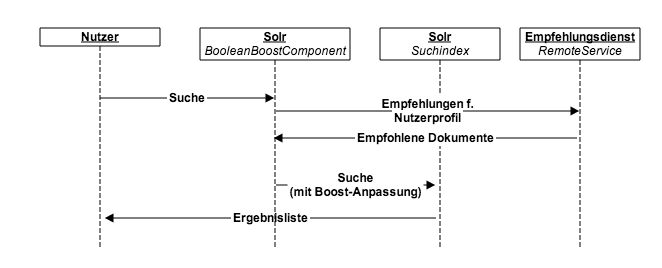
\includegraphics[width=\textwidth]{Abbildungen/search-rec1.png}
    \caption[Flussdiagram - externe Empfehlungen]{\footnotesize Flussdiagramm: Personalisierung von Suchanfragen über einen externen Empfehlungsdienst.}
    \label{fig:seq-extern-recommender}
\end{figure}

Wie in \ref{fig:seq-extern-recommender} dargestellt, wird die ursprüngliche Suchanfrage des Nutzers innerhalb der Komponente zunächst unterbrochen, um für das entsprechende Nutzerprofil die Empfehlungen vom externen Dienst berechnen zu lassen. Enthält die Antwort des Dienstes eine Liste von Empfehlungen, so wird diese innerhalb der Komponente in eine Solr-Anfrage, in diesem Fall einen \textit{BooleanQuery}, umgewandelt. Innerhalb des \textit{BooleanQuery} wird über \textit{TermQuery}-Elemente jeweils die Empfehlung für ein einzelnes Dokument der entsprechenden Solr-DokumentenID zugeordnet. Die so generierte Liste wird mit der ursprünglichen Anfrage verknüpft und entsprechend weiterverarbeitet. Die Kombination beider Anfragen hat dann zur Folge, dass Dokumente aus den Empfehlungen über die Faktoren des \textit{TermQuery} entsprechend ``besser'' bewertet werden wenn sie in der Ergebnisliste der ursprünglichen Suchanfrage enthalten sind. Sind die empfohlenen Dokumente nicht Teil der Ergebnisliste, kann keine Personalisierung vorgenommen werden und die Gewichtung bzw. Sortierung der Ergebnisse erfolgt rein TF-IDF-basiert.

Zur Konfiguration der Komponente stehen folgende Parameter zur Verfügung:
\begin{itemize}
\item \textit{boostBase} - Normalisierungswert bei der Dokumentenboost-Berechnung. ( $\alpha$ aus Formel (\ref{form:myscore0}) ).
\item \textit{boostAmount} - Menge der zu bildenden Empfehlungen
\item \textit{boostInline} - Schaltet die Integration in die ursprüngliche Anfrage ab und zeigt nur die Empfehlungen.
\end{itemize}

Die Verarbeitung kann hierbei komplett in der Vorverarbeitungsphase von Apache Solr erfolgen, so dass die eigentlichen Suchanfragen auch von innerhalb von Solr in Zwischenspeichern gehalten werden können und wiederholte Anfragen erbeblich schneller verarbeitet werden können.

\subsubsection{Integrierte Empfehlungsdienste} \label{sec:implmodelcalc}

Die Implementierung von Empfehlungen mit Hilfe von Element-Featurevekoren, wurde innerhalb der \textit{SimilarityBoost}-Komponente implementiert.  Die Verarbeitung einer Suchanfrage wird in Abbildung  \ref{fig:seq-intern-recommender} dargestellt.

\begin{figure}[H]
  \centering
    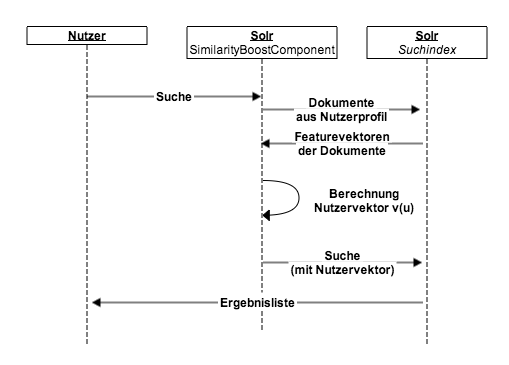
\includegraphics[width=0.77\textwidth]{Abbildungen/search-rec2.png}
    \caption[Flussdiagram - interne Empfehlungsbildung]{\footnotesize Flussdiagramm: Personalisierung von Suchanfragen über Featurevektoren im Suchindex.}
    \label{fig:seq-intern-recommender}
\end{figure}

Nachdem die Komponente die Anfrage des Nutzers erhalten hat, muss zunächst über eine zusätzliche Anfrage, die Liste der Dokumente des Nutzerprofils aus dem Suchindex gelesen werden. Mit Hilfe dieser Liste kann dann, der Nutzervektor $v(u)$ wie in Formel \ref{form:anonuser} gebildet werden. Danach kann die ursprüngliche Anfrage weiterverarbeitet werden.

Da die Konfiguration der Komponente (vgl. Listing \ref{lst:similardocs}) die weitere Verarbeitung von $v(u)$ (im Listing als \textit{\$features} bezeichnet) bestimmt, kann die Personalisierung bzw. Empfehlungsbildung unabhängig von der \textit{SimilarityField}-Komponente erfolgen. Das in Listing \ref{lst:similardocs} gezeigte Beispiel nutzt die Distanz zwischen den Dokumentenvektoren $w(i)$ und dem Nutzervektor $v(u)$ um für den Nutzer relevante Dokumente zu bevorzugen.

Da der größte Teil der Empfehlungsbildung innerhalb der normalen Apache Solr Komponenten erfolgt, beschränkt sich die Konfiguration der \textit{SimilarityField}-Komponente auf die Benennung des Featurevektoren-Feldes über den \textit{similarityField} Parameter. Alle weiteren Verarbeitungsschritte und Parameter werden innerhalb der \textit{solrconfig.xml} direkt angegeben.

\subsection{Systemaufbau}

Für die in Abbildung \ref{fig:system_rough} skizzierten Systembestandteile wird im Folgenden die gewählte Technologie erläutert und mit möglichen Alternativen verglichen.

\subsubsection{Tracker} \label{sec:tracker-impl} Die Aufzeichnung der Interaktionen von Nutzer und Webseite, wurde mit Hilfe eines eigenen Java \glslink{Servlet}{Servlets} umgesetzt. Die Funktionalität des Trackers beschränkt sich auf das Erfassen von Interaktionen eines Nutzers innerhalb einer JavaScript-Bibliothek und die Weitergabe dieser innerhalb des Servlets. Da die Daten dem Anwendungsfall entsprechend gespeichert werden können, ist der Aufwand bei der weiteren Verarbeitung sehr gering.

Da ein ``Datensatz'' einer Komponente der in Tabelle \ref{tab:user-item-ratings} gezeigten Matrix entspricht, enthält dieser auch ähnliche Daten. Für den Nutzer wird jeweils eine ID für die aktuelle Session, eine sessionübergreifende ID und (falls bekannt) den Account im System aufgezeichnet. Für das Element bzw. Produkt wird die \gls{SKU-ID} aufgezeichnet und ggf. eine Produktgruppen-\gls{ID}. Die Information über die Art der Interaktion wird in textheller Form gespeichert. In der Summe besteht ein einzelner Datensatz so aus ca. 114-150 Byte. Die Weitergabe dieser Daten erfolg über die im Abschnitt \ref{sec:datatransp} beschriebene Transporttechniken. Der Quellcode der Komponente ist unter \todo{Reg zum Tracker-Repo} verfügbar.

Wichtigste Alternative zur Implementierung eines eigenen Dienstes wäre die Nutzung bzw. Auswertung schon vorhandener Daten aus Serverlogs und von externen Trackingdiensten (zB. Google Analytics) gewesen. Da dies allerdings mit sehr hohen Aufwand bei der Datenaufbereitung verbunden wäre und da nicht in jedem Anwendungsfall auf entsprechende Logs zurückgegriffen werden kann, wurde auf diese Art der Datengewinnung zunächst verzichtet.

\subsubsection{Datenhaltung} Für die dauerhafte Speicherung der aufgezeichneten Daten wurde zunächst auf die Verwendung eines verteilten Dateisystems (vgl. Abschnitt \ref{sec:hfs}) verzichtet. Da der Betrieb eines entsprechenden Serverclusters hohe Wartungskosten erzeugt hätte, wurde die lokale Speicherung der Daten und die bedarfsgemäße Nutzung von Amazon Web Services gewählt. Dies ermöglicht die MapReduce-basierte Verarbeitung der Daten (vgl. Abschnitt \ref{sec:mapred}) ohne dedizierte Hardware vorhalten zu müssen.

Der Kostenunterschied kann mit Hilfe der folgenden Rechnung veranschaulicht werden. Geht man von 50GB an aufgezeichneten Nutzdaten pro Jahr aus, erzeugt die Speicherung dieser Datenmenge zur Verarbeitung innerhalb des \textit{Amazon Simple Storage Services} (S3) Kosten von ca. \EUR{6} pro Transfer (Upload+Download). Würde man zur weiteren Verarbeitung drei \textit{Amazon Elastik Compute Cloud} \textit{m2.xlarge} Instanzen für einen Tag nutzen, entstünden Kosten von ca. \EUR{100} pro Tag \footnote{Als Vergleichswert wurde die unter http://calculator.s3.amazonaws.com/calc5.html am 01.08.2013 gezeigten Tagespreise genutzt}. Die Kosten von wöchentlichen Neuberechnungen innerhalb dieser Infrastruktur entsprechen damit ca. der Hälfte der anfallenden Kosten zur Anmietung ähnlicher Ressourcen bei normalen Hosting-Anbietern.

\subsubsection{Datentransport} \label{sec:datatransp} Zum sicheren Transport der Daten zwischen Tracker und der Datenhaltung wird \textit{Apache Flume} genutzt. Es implementiert ein einfaches \textit{Message Queue} System welches sicherstellt, dass alle Daten einer Quelle (Tracker) auch auf allen Senken (Datenhaltung) geschrieben wurden bevor diese das System verlassen. Im Vergleich zur direkten Speicherung der Daten auf einer entsprechenden Festplatte, bietet Apache Flume die Möglichkeit mit mehrere Quellen oder mehrere Senken zu arbeiten und Datenströme zu verteilen bzw. zusammenzufassen. Neben dem lokalen Dateisystem unterstützt Apache Flume zudem auch HDFS-Senken und Amazon S3-Senken. Dank dieser Eigenschaften wird sowohl die horizontale Skalierung des Trackers auf mehrere Knoten vereinfacht, als auch die Anbindung anderer, dem Anwendungsfall entsprechender, Datenhaltungssysteme.

Alternative Message Queue Systeme wie etwas Rabbit MQ oder Active MQ wurden nicht betrachtet.

\subsubsection{Datenaufbereitung} Die Vorverarbeitung der Daten wurde mit \textit{Apache Pig} umgesetzt. Es stellt eine dem Anwendungsfall angepasste Datenflusssprache, das sog. \textit{Pig Latin}, zur Verfügung (Beispiel siehe Listing \ref{lst:pigprofiles}). Die darin beschriebenen Operationen werden zur Verarbeitung in \textit{Apache Hadoop} kompatible \textit{MapReduce} Operationen kompiliert und sind so ohne weitere Anpassungen verteilt ausführbar.  Damit ermöglichht es, die Anwendung der in Abschnitt \ref{sec:mapred} beschriebenen Methoden um Skalierbarkeit zu gewährleisten. Die in \textit{Pig Latin} beschriebenen Datenverarbeitungsprogramme lassen sich über \textit{Amazon Elastic MapReduce} auch für Daten nutzen welche in \textit{Amazon S3} gehalten werden. \citep{Lin2012}

 \lstinputlisting[caption=Apache Pig Beispielscript zur Kombination von Nutzerprofiledaten,float,language=bash,label={lst:pigprofiles}]{Listings/pig-profiles.txt}

Eine umfassende Dokumentation der Möglichkeiten von \textit{Apache Pig} zur Datenverarbeitung bietet \citep{gates2011programming}. Die Integration von Aufgaben des maschinellen Lernens mit  \textit{Apache Pig} wird in  \citep{Lin2012} beschrieben.

Alternative \textit{MapReduce} Implementierungen in Java oder \textit{Apache Hive} wurden nicht betrachtet.

\subsubsection{Empfehlungsdienst} Wie im vorangegangen Abschnitt \ref{sec:mahout} beschrieben, wurde die Integration der Empfehlungs- und Modellberechnung mit \textit{Apache Mahout} vorgenommen.

Die Vorberechnung der Ähnlichkeitsmodelle (vgl. Abschnitt \ref{sec:scalefiltering}) wird als verteilte Berechnung wie in Listing \ref{lst:useritemmodelprep} ausgeführt. Um die darin berechneten Modelle direkt im Empfehlungsdienst nutzen zu können, wird die Ähnlichkeitsmatrix in einem Nachverarbeitungsschritt (vgl. \textit{PairSimilarityJob}) in ein textuelles Austauschformat überführt. Dieses Austauschformat wird dann über das in Mahout vorhandene \textit{FileDataModel} in den Empfehlungsdienst geladen. Dieser wird als Webservice über eine HTTP-Schnittstelle (vgl. \textit{com.aoe.cf.recommender.RemoteService}) zur Verfügung gestellt. Die Matrixfaktorisierung wird wie in Listing \ref{lst:factorgenerator} gezeigt, mit den in Abschnitt \label{sec:myrecommend} beschriebenen Methoden durchgeführt.

Die Evaluation der Ergebnisse beider Vorberechnungsmethoden erfolgt über die ergänzend bereitgestellten Evaluationsprogramme. In beiden Fälle werden die Empfehlungsergebnisse für zuvor gespeicherten Testdaten (vgl. Listing \ref{lst:dataprep}) mit den tatsächlich bekannten Daten vergleichen um die in Abschnitt \ref{sec:measures} beschriebenen Metriken zu generieren.

\subsubsection{Suche}

Die Integration mit der Suche erfolgt wie in Abschnitt \ref{sec:searchrelevance} beschrieben. Die Empfehlungsdienste auf Basis des Webservices werden wie in Listing \ref{lst:solrconfig} über die \textit{booleanBoost}-Komponente eingebunden und konfiguriert. Zur Integration der featurebasierten Empfehlungen wird die \textit{similarityField} Komponente eingebunden und über die erweiterte Boost-Konfiguration wie in Listing \ref{lst:similardocs}  zur Personalisierung benutzt.

Zur Erfüllung der in Abschnitt \ref{sec:userstories} beschriebenen Anwendungsfälle können beide Komponenten auch so integriert bzw. konfiguriert werden, dass Empfehlungen direkt ``ausgegeben'' werden oder dass Empfehlungen nicht für reale Nutzerprofile und stattdessen für anonyme Produktlisten generiert werden. Da beide Komponenten direkt in den Verarbeitungsablauf von \textit{Apache Solr} integriert sind, obliegt die Ausgestaltung der konkreten Anwendungsfälle der konkreten Applikation und wird zur Wahrung des Umfangs nicht näher betrachtet.

%\subsubsection{Datenhaltung}
%\subsection{Systemaufbau}
%\subsubsection{Tracking-Pixel}
%\subsubsection{Datenhaltung}
% Siehe "Programming Pig" S 19.2
%\sub
